\section{Alloy}
This section is dedicated to the Alloy model of the CodeKataBattle software, included all the functions of the application and their most important constraints. 
\newline
In this model, we want to prove that:
\subsection{Signatures}

\begin{lstlisting}
//Definition of the Student
sig Student {
}

//Definition of the Educator
sig Educator {
}

//Definition of the Tournament
sig Tournament {
	   creator: one Educator,                 
	   invitedEducators: set Educator,   
	   participantEducators: set Educator,  
	   Battles: disj some Battle, 
	   participantStudents: set Student   
} 

//Definition of the Battle
sig Battle {
 	 creator: one Educator,                       
  	 participantTeams: set Team,             
	 evaluator: disj one Evaluator,            
	 has: disj one FinalRankingBattle    
}

//Definition of the Team
sig Team {
	 creator: one Student,                         
	 members: set Student,                       
	 push: disj set Project,                     
	 lastPush: disj lone LastProject         
}

//Definition of the Evaluator
sig Evaluator{
	configurator: one Educator              
} 

//Abstract definition of a project
abstract sig Proje {
	 rated: one Evaluator,                  
	 has: disj one Score                   
}

//Definition of a Project
sig Project extends Proje{

}

//Definition of a LastProject
sig LastProject extends Proje{
	 manualEvaluation: lone Educator
}

//Definition of a Score 
sig Score {
}

//Definition of a FinalRankingBattle
sig FinalRankingBattle{
	 basedOn: set Score         
}

\end{lstlisting}


\clearpage
\subsection{Facts}

\begin{lstlisting}

//All final battle rankings have a battle in which the following participate
fact EachFinalRankingBelongsToBattle{
all rb: FinalRankingBattle | one b: Battle | rb in b.has 
}


// The final battle ranking is based on the scores of the last projects pushed 
fact FinalRankingBasedOnScores{
all rb: FinalRankingBattle, b: Battle | rb in b.has implies  rb.basedOn =  b.participantTeams.lastPush.has 
}


//Evaluator can only be configured by the creator of the battle where the team participates 
fact EvaluatorConf{
	all ev: Evaluator, b: Battle | ev in b.evaluator implies ev.configurator = b.creator
}

//A team's pushed project is evaluated by the evaluator who has the battle where the team is enrolled
fact ProjectRated{
	all p: Proje, tm: Team,  b: Battle | tm in b.participantTeams and (p in tm.push or p in tm.lastPush) implies p.rated =  b.evaluator
}

//The educator who created the battle can decide whether or not to do manual evaluation of the teams' latest projects 
fact SameManualEvaluationInBattle {
  all b: Battle |
      all lp1, lp2: LastProject |
        (lp1 in b.participantTeams.lastPush and lp2 in b.participantTeams.lastPush) implies
          lp1.manualEvaluation = lp2.manualEvaluation or no lp1.manualEvaluation 
}

//This facts allows us to say that if one team has the last project delivered the others will have it too because the battle will be over
fact LastProjectConsistency {
 all b: Battle | #b.participantTeams.lastPush > 0 implies #b.participantTeams =  #b.participantTeams.lastPush
}


//All the latest projects have a Team where the following are included.
fact LastProjectInTeam{
all p: LastProject | one tm: Team|  p in tm.lastPush
}

//All the projects have a Team where the following are included.
fact ProjectInTeam{
all p: Project | one tm: Team|  p in tm.push
}

//All the scores have a project where the following are included.
fact ScoreInProje{
all sc: Score | one pj: Proje | sc in pj.has
}

//All the Evaluator have a Battle where the following are included.
fact EvaluatorInBattle{
all e: Evaluator | one b: Battle|  e in b.evaluator
}

//All the Battle have a Tournament where the following are included.
fact BattleInTournament{
all b: Battle | one t: Tournament|  b in t.Battles
}

//All the Team have a Battle where the following are included.
fact TeamInBattle{
all tm: Team | one b: Battle|  tm in b.participantTeams
}

//A battle in the tournament implies that the creator of the battle must be part of the tournament educators and the participants of the battle must be part of the tournament
fact EachBattleBelongsToOneTournament {
  all t: Tournament, b: Battle |
    (b in t.Battles) implies (b.creator in t.participantEducators and b.participantTeams.members in t.participantStudents)
}

//A team can only participate in one battle at a time 
fact TeamBattaglia {
all disj b1, b2: Battle, tm: Team | tm in b1.participantTeams implies tm not in b2.participantTeams
}

// Each team has some students within
fact StudentCanParticipateInOneTeam {
  all tm: Team | some s: Student | s in tm.members
}

//A student may participate in one team at a time
fact NoDuplicateStudentAcrossTeam {
  all disj t1, t2: Team, s: Student | s in t1.members implies s not in t2.members
}


//The creator educator is part of the tournament participants
fact CreatorPartecipate {
  all t: Tournament, e: Educator | e in t.creator implies e in t.participantEducators and e not in t.invitedEducators
}

//Only invited eductors can be participants 
fact OnlyInvitedEducatorsCanParticipate {
  all t: Tournament, e: Educator | e in t.participantEducators and e not in t.creator implies e in t.invitedEducators
}


//All educators participating in the tournament create at least one battle 
fact EducatorParticipatesInBattleCreateAtLeastOneBattle {
  all e: Educator, t: Tournament |
    e in t.participantEducators implies some b: Battle | b in t.Battles and b.creator = e
}


//The creator of a team is part of the members of the same team
fact CreatorIsMemberOfTeam {
  all tm: Team | tm.creator in tm.members


//A general scenerio of the system
pred createScenario {
	#Educator = 2

	#Student = 5

	#Tournament = 1

	#Battle = 2

	#Team = 3

	#LastProject > 1

	#Project > 1
}


run createScenario for 5


  
}

\end{lstlisting}

\clearpage

\begin{landscape}
\begin{figure}[h]
    \centering
    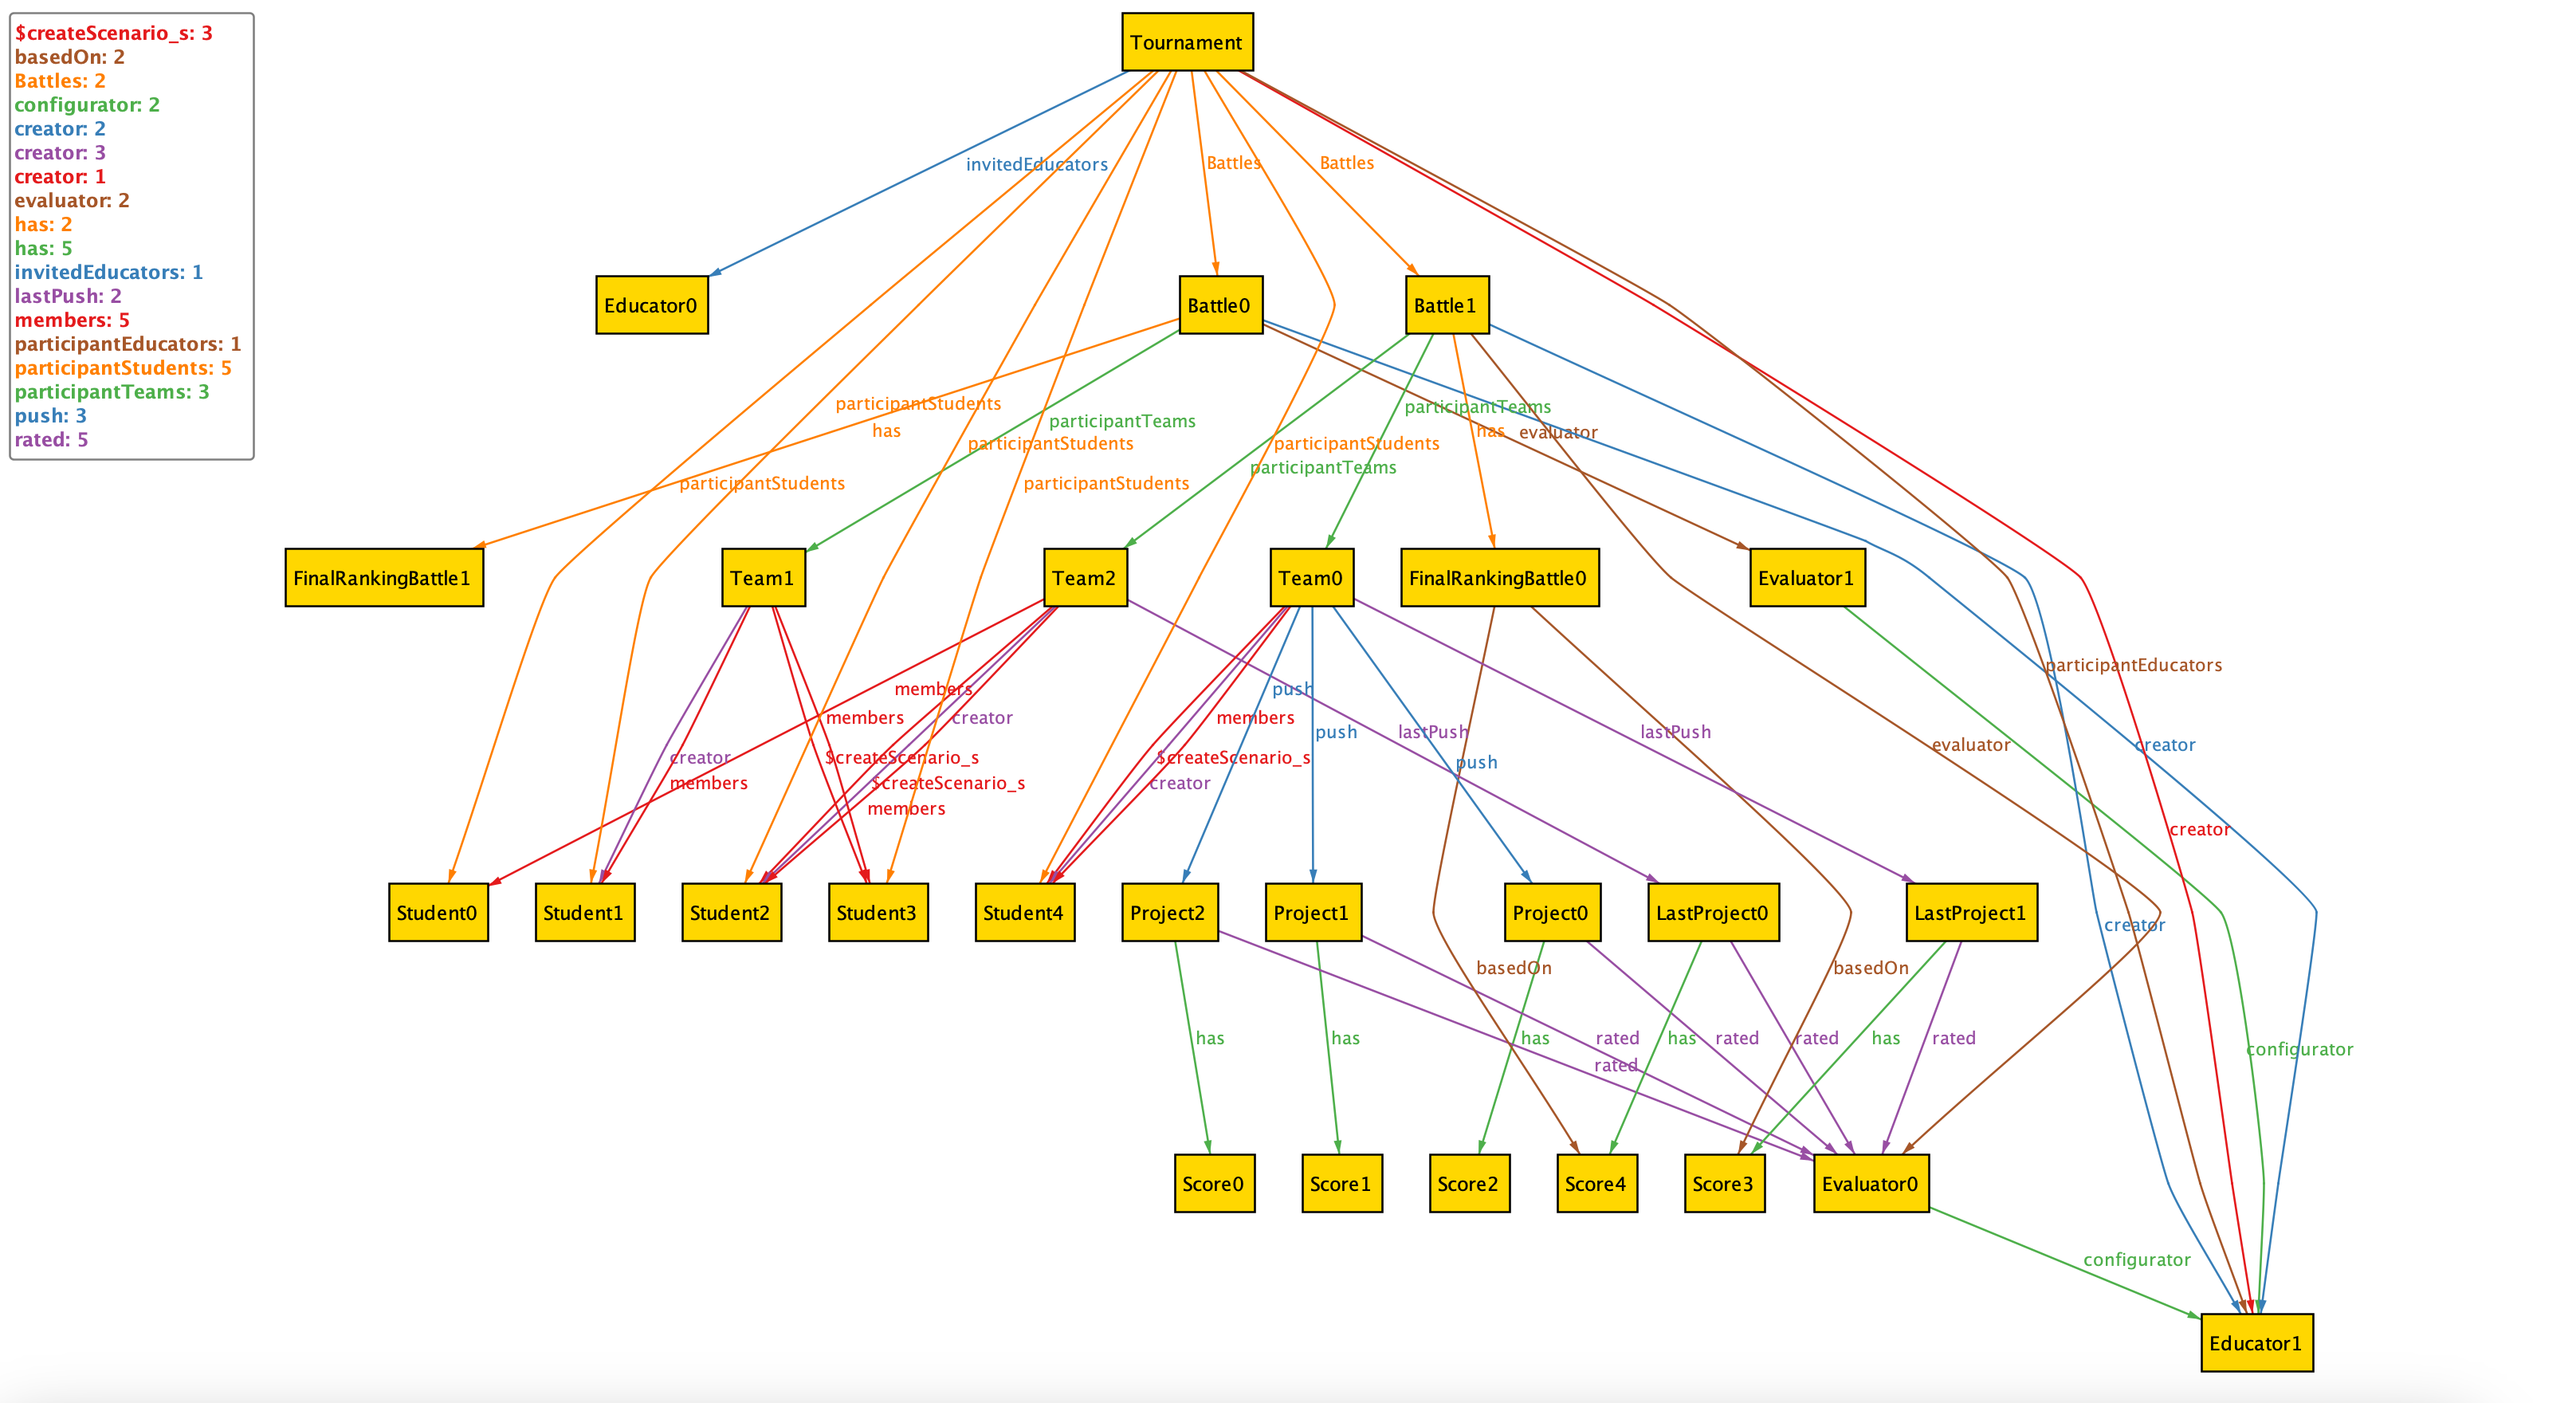
\includegraphics[scale=0.5]{images/AlloyView.png} 
    \label{fig_PushGitHubSD}
\end{figure}
\end{landscape}

\clearpage

\begin{comment}
In questa immagine possiamo vedere uno scenario generico del sistema. Partendo dall'alto notiamo che è presente un istanza torneo a cui sono collegate alcune relazione, la prima che notiamo è un invitedEducator, questa relazione significa che l'educator0 è stato invitato a partecipare al torneo ma siccome non c'è una relazione di participantEducators, vuol dire che l'educator ha rifiutato l'invito di partecipazione. Poi a destra notiamo due relazione che sono participantEducators e creator che sono le relazione che lega il torneo al Educaotr che ha creato il torneo, poi vediamo che ha al suo interno 2 battaglie e ha in particolare 5 studenti iscritto al torneo. Le due istanze battaglie possiamo notare che sono diverse fra loro siccome la battaglia0 partecipa solo il team1 con al suo interno due studenti (Student1 e Student3) dove si può vedere dalla relazione creator che Student1 è il creatore del team. Notiamo che questo team non ha ancora effatuato nessuno push di progetti siccome il team non ha nessuna relazione riguardante. Poi ovviamente la battaglia ha un valutatore che è configurato dall'educator che creato la battaglia. In fine la battaglia0 ha una classifica della battaglia finale che al momento è vuota siccome la battaglia sarà ancora in corso. 
Mentre la battaglia1 che contiene il team2 e il team0,  ha le stesse caratteristiche dell'altra battaglia ma in questo caso i due team hanno effettuato il loro push e in particolare hanno consegno il loro ultimo progetto, ogni progetto in questo caso è valutato dal valutatore configurato dall'educator che ha creato la battaglia, ma l'ultimo progetto può essere valutato manualmente dall'educator che ha creato la battaglia, ma in questo caso non è avvenuto. In fine vediamo che la classifica finale della battaglia0 si basa sugli score ottenuti dagli ultimi progetti consegnati dai due team.
\end{comment}


In this schematic representation of the system, we can observe a generic tournament instance with connections to several relationships. From above we notice that there is a tournament instance connected to several relationships. The first relationship highlighted is invitedEducator, which indicates that educator0 has been invited to participate in the tournament. However, since there is no participantEducators relationship, we can infer that the educator declined the invitation to participate.
\vspace{1\baselineskip}
\newline
Next, we notice two relationships, participantEducators and creator, that link the tournament to the educator who created it. Also, we see that the tournament contains two battles and has 5 students enrolled. The two instances of the battles are different from each other. For example, battle0 has only team1 as a participant, which includes students Student1 and Student3. This team has not yet done any project push, as indicated by the lack of project-related reports.
\vspace{1\baselineskip}
\newline
Next, we observe battle1, which contains team2 and team0. Both teams have pushed their projects, including the last delivered projects. Each project is evaluated by the evaluator configured by the educator who created the battle. A manual evaluation by the battle creator of the last project is also possible, but in this case it did not happen. Finally, we note that the final battle ranking1 is based on the scores obtained from the last projects delivered by the two teams.




